\chapter{Project Management} \label{management}
% List project objectives
% Define project goal clearly
% - Create standalone Java program that can convert SBML files into the format of ERODE
% - The program should also be able to translate ERODE output back into SBML
% - Add support for both BNs and multi-valued networks in the converter
% - Integrate the converter into ERODE
Managing a project is just as important as working on the project itself, as is allows to direct the project towards a designated goal. For this project the first step was to divide it into several stages. For each stage, a milestone was defined, declaring what should be achieved during that stage. During the project, some of the original milestones eventually had to be abandoned, as it for example was discovered that the available tools were unable to achieve the desired result or that the amount of work required would extend far beyond the project's time frame. Specifically, the milestone to add support for the conversion of multi-valued networks (MNs) had to be abandoned, because ERODE's developers were unable to add support for MNs within the time-frame of this project.

The following list contains all milestones that were kept until the end of the project:
\begin{itemize}
    \item \textbf{Familiarize with SBML and the JSBML-library.} In order to. eventually, create a converter between SBML and ERODE, it is required to understand how biological models are represented in SBML. The same goes for the JSBML-library as it is a library used to represent SBML-models in Java.
    
    \item \textbf{Create a few small JSBML demos, that can extract data from SBML files.} These demos were used as small stepping stones, towards the construction of the converter and an opportunity to experiment with the JSBML-library.
    %\comg{the first one refers to the Qualitative modelling of the network controlling Trp biosynthesis \url{http://ginsim.org/node/50}, the second one refers to cortical area development (CAD), and the third refers to "let's find a third one"}
    \item \textbf{Create a prototype SBML converter that can generate ERODE-files from an SBML-qual input.} In this first stage, the aim was to develop a basic framework for the conversion, a proof of concept for the later stages of the converter.
    \item \textbf{Extend the prototype to support all kinds of BNs by adding support for all Boolean operators supported by SBML.} 
    
    \item \textbf{Extend the prototype to support conversion from ERODE to SBML.}
    \item \textbf{Test changes and added features during development.} This is required to ensure a correct conversion between the two models representations. By testing each newly added feature and ensuring that the previously added tests still succeeds,  this can be verified.
    
    \item \textbf{Extract the core functionality to a Java-library to support integration into other projects.} By decoupling the core functionality of the converter from its program shell, the library could be used as a plugin in other projects. As an example, the converter could be integrated into ERODE, to allow direct importing and exporting of SBML-files.
    
\end{itemize}

To achieve these milestones the project was planned, and its progress tracked, on two different levels. On project level, the milestones and a few larger tasks were  planned and monitored using a Gantt-chart to visualize the overall progression. Additionally, weekly meetings with the supervisors were used to plan and track the progress of the individual milestones.
\begin{figure}[H]
    \centering
    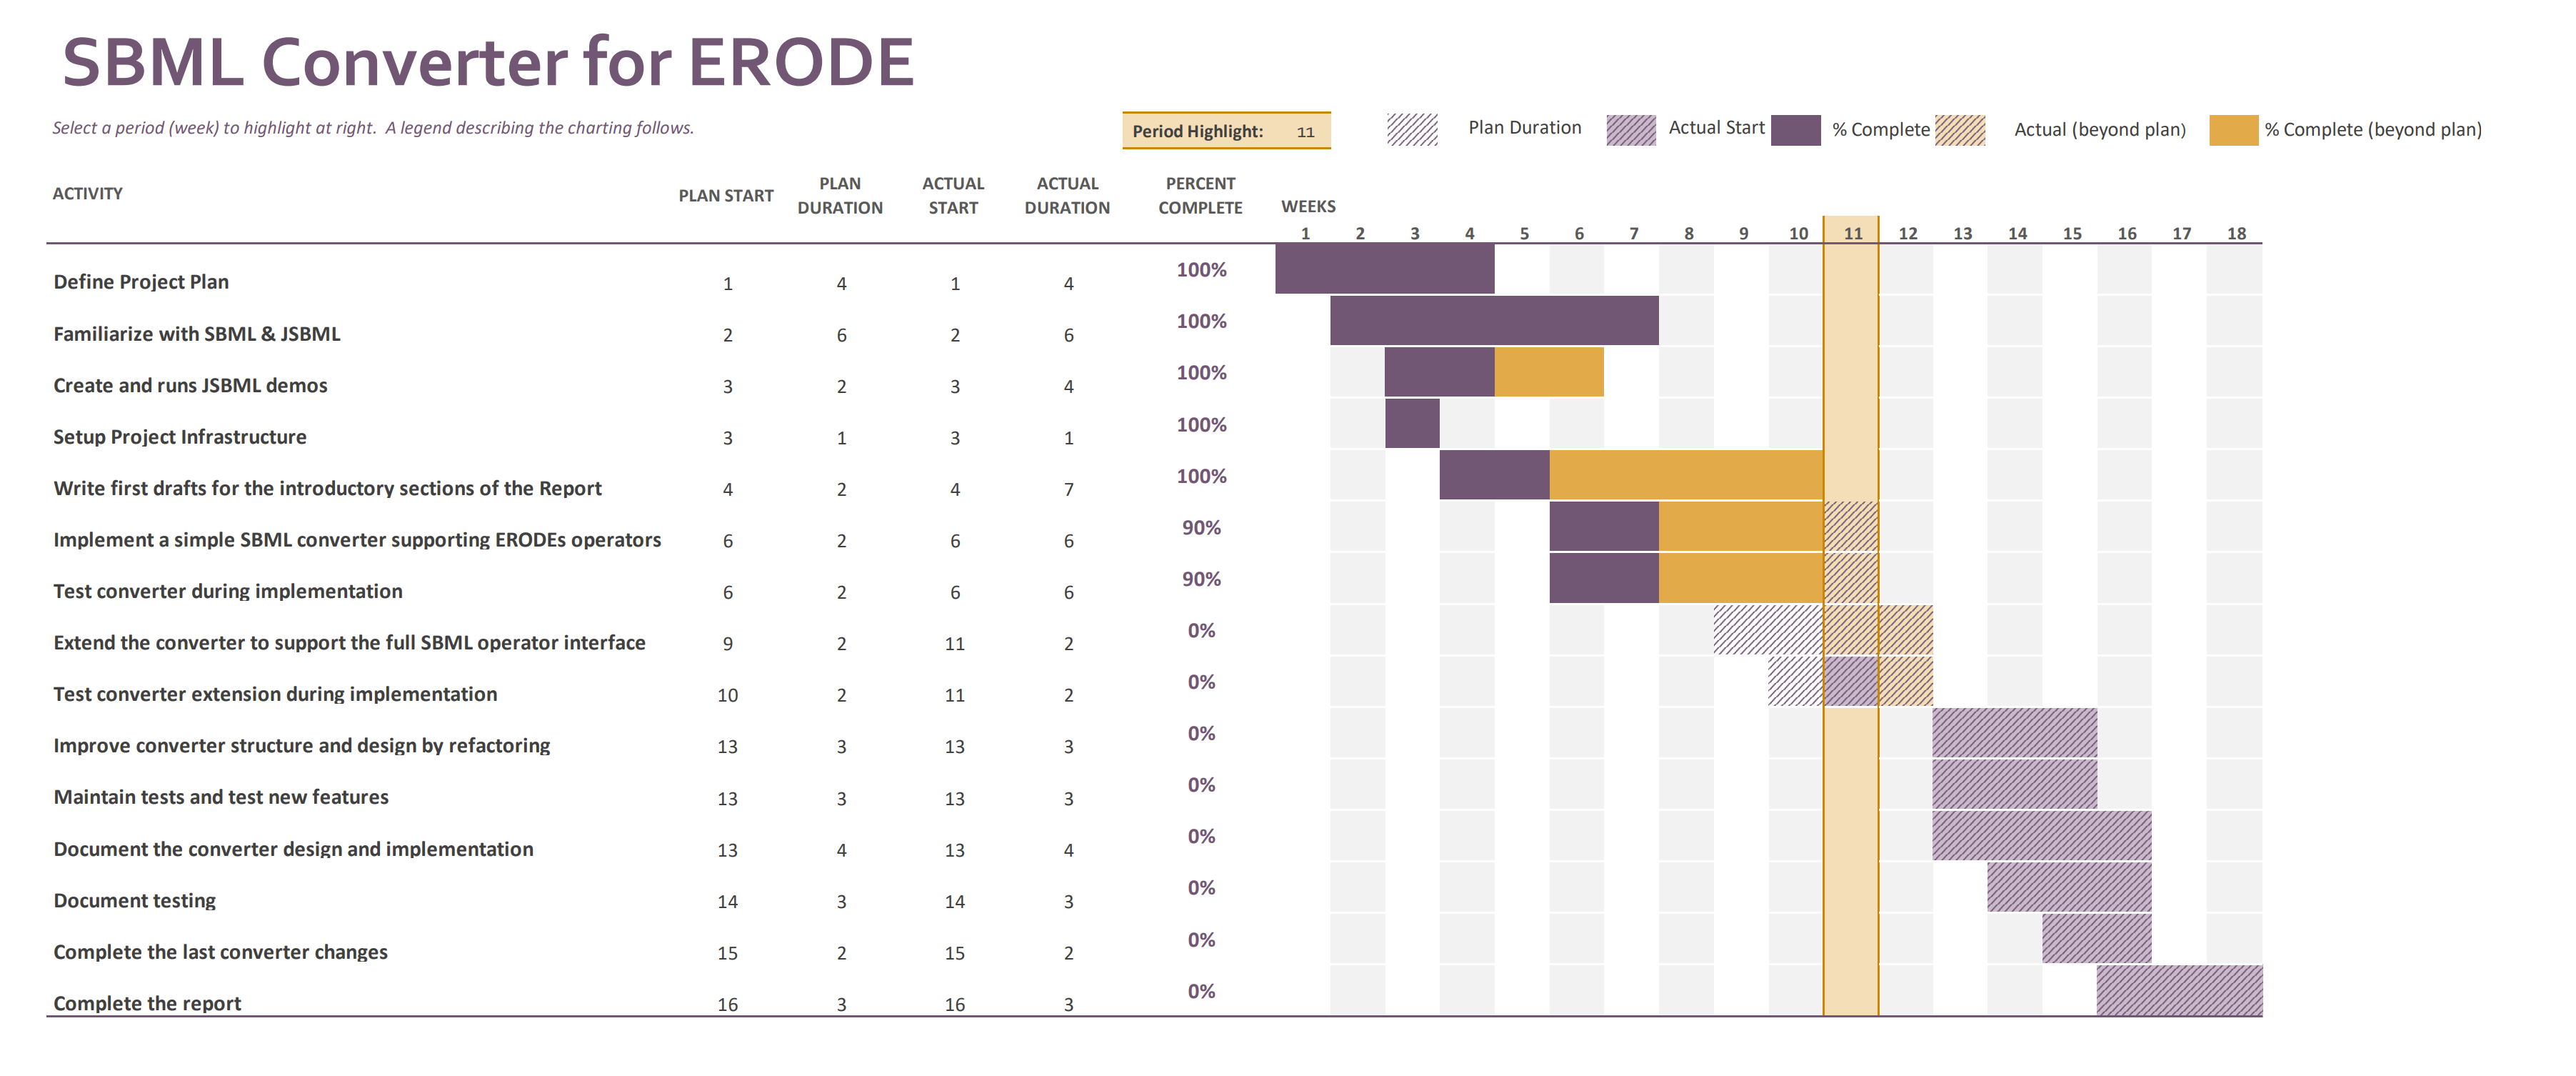
\includegraphics[scale=0.38]{Sections/Images/Project Plan.jpg}
    \caption{Gantt chart used to track the project's progress}
    \label{fig:gantt}
\end{figure}
The project code was managed using GitHub as a version control system and the Apache Maven (\cite{porter_zyl_lamy}) development tool as a code management for Java-projects (see section 3).
The \href{https://github.com/Unfunctioned/SBML-Converter-for-ERODE}{GitHub repository} can be found at \url{https://github.com/Unfunctioned/SBML-Converter-for-ERODE}.
%The next step was then to manage the required time for each milestone. This was achieved by 
%Since time is a limited resource for this project, it needs to be managed as one.\comg{?} To do so project management is required, which for this project needs to cover three different aspects.

%\begin{enumerate}
%    \item \textbf{Planning} as a means to direct the project towards its intended goal.
%    \item \textbf{Progress tracking} in order to monitor resources and adjust planning according to their changes.
%    \item \textbf{Code Management} in order to maintain a simple and efficient workflow.
%\end{enumerate}
%The planning and progress tracking of the project has been executed on two different levels. On a more abstract level the major project objectives have been planned and tracked using a Gantt-chart to give a general overview of the entire project and track its progress. On a more detailed level, weekly meetings with the supervisors have been used to plan and track the progress of the individual tasks that make up each objective on a week-to-week basis.
%\begin{comment}
%INSERT GANTTCHART HERE
%\end{comment}

%The project code has been managed using Git as a version control system (VCS) and Apache Maven to simplify the development workflow of the Java-project.

%The GitHub-repository can be found at: \verb+INSERT LINK HERE+


\begin{comment}
Project Management:
- Planning
- Code management
- Progress tracking
\end{comment}



%Present project plan with graphics
%Kanban boards for details task tracking
% - Those were later discontinued, due to giving little to no management benefit
%Apache Maven
% - Move tool section here!